\documentclass[10pt,a4paper]{article}

\usepackage[a4paper,top=18mm,bottom=19mm,left=19mm,right=19mm]{geometry}
\usepackage{fontspec}
\usepackage{microtype}
\usepackage[table]{xcolor}
\usepackage{booktabs}
\usepackage{tabularx}
\usepackage{array}
\usepackage{siunitx}
\usepackage{tikz}
\usetikzlibrary{arrows.meta,calc,positioning,fit,backgrounds}
\usepackage{pgfplots}
\pgfplotsset{compat=1.18}
\usepackage[most]{tcolorbox}
\usepackage{enumitem}
\usepackage{titlesec}
\usepackage{fancyhdr}
\usepackage{hyperref}
\usepackage{caption}
\usepackage{float}
\usepackage{lastpage}
\usepackage{ragged2e}
\usepackage{setspace}

\setmainfont{Calibri}
\setsansfont{Calibri}
\setmonofont{Consolas}
\renewcommand{\familydefault}{\sfdefault}

\definecolor{Ink}{HTML}{17202A}
\definecolor{Muted}{HTML}{5D6D7E}
\definecolor{Rule}{HTML}{D6DBDF}
\definecolor{Teal}{HTML}{1F7A8C}
\definecolor{Red}{HTML}{B03A2E}
\definecolor{Purple}{HTML}{7D3C98}
\definecolor{Gold}{HTML}{B7950B}
\definecolor{Green}{HTML}{287D3C}
\definecolor{SoftGray}{HTML}{F4F6F7}
\definecolor{SoftRed}{HTML}{FDEDEC}
\definecolor{SoftTeal}{HTML}{E8F6F8}
\definecolor{Slate}{HTML}{6C7A89}
\definecolor{CoverCharcoal}{HTML}{222426}
\definecolor{CoverInk}{HTML}{191B1D}
\definecolor{CoverMuted}{HTML}{666A6E}
\definecolor{CoverRule}{HTML}{C8C9C7}
\definecolor{CoverSoft}{HTML}{F3F3F1}

\hypersetup{
  colorlinks=true,
  linkcolor=Teal,
  urlcolor=Teal,
  citecolor=Teal,
  pdftitle={Trump Occurrence Forecasting Benchmark: Technical Report},
  pdfauthor={Ashish Pandey},
  pdfsubject={48-hour offline forecasting benchmark},
  pdfkeywords={forecasting, transcript occurrence, calibration, Brier score, chronological evaluation}
}

\titleformat{\section}
  {\Large\bfseries\color{Ink}}
  {\thesection}{0.65em}{}
  [\vspace{1mm}\color{Rule}\titlerule]
\titleformat{\subsection}
  {\large\bfseries\color{Ink}}
  {\thesubsection}{0.55em}{}
\titlespacing*{\section}{0pt}{8pt}{7pt}
\titlespacing*{\subsection}{0pt}{7pt}{4pt}

\setlength{\parindent}{0pt}
\setlength{\parskip}{4.5pt}
\setcounter{tocdepth}{1}
\setlist[itemize]{leftmargin=5mm,itemsep=2pt,topsep=3pt}
\setlist[enumerate]{leftmargin=6mm,itemsep=2pt,topsep=3pt}
\renewcommand{\arraystretch}{1.18}
\sisetup{
  round-mode=places,
  round-precision=6,
  detect-all,
  table-number-alignment=center
}

\pagestyle{fancy}
\fancyhf{}
\fancyhead[L]{\small\color{Muted}Trump Occurrence Forecasting Benchmark}
\fancyhead[R]{\small\color{Muted}Technical Report}
\fancyfoot[L]{\small\color{Muted}Ashish Pandey}
\fancyfoot[R]{\small\color{Muted}\thepage\ of \pageref{LastPage}}
\renewcommand{\headrulewidth}{0.4pt}
\renewcommand{\footrulewidth}{0pt}

\newcommand{\metric}[1]{\textbf{\color{Ink}#1}}
\newcommand{\code}[1]{\texttt{\small #1}}
\newcommand{\BaselineBrier}{0.043319}
\newcommand{\ChallengerBrier}{0.044434}
\newcommand{\BlankedBrier}{0.044460}
\newcommand{\ConstantBrier}{0.048416}
\newcommand{\DeltaBrier}{0.001115}
\newcommand{\RelativeWorse}{2.58\%}
\newcommand{\DeltaLow}{0.000259}
\newcommand{\DeltaHigh}{0.002074}
\newcommand{\PackageHash}{B7DC0E2D84241AC7716286313807753B88C54EFE295B19808D02DD04C5E4EC0E}

\newtcolorbox{decisionbox}{
  enhanced,
  colback=SoftRed,
  colframe=Red,
  boxrule=0.8pt,
  arc=1.5mm,
  left=4mm,right=4mm,top=3mm,bottom=3mm
}

\newtcolorbox{insightbox}[1]{
  enhanced,
  colback=SoftTeal,
  colframe=Teal,
  boxrule=0.6pt,
  arc=1.5mm,
  title=\textbf{#1},
  coltitle=Ink,
  fonttitle=\bfseries,
  left=3.5mm,right=3.5mm,top=2.5mm,bottom=2.5mm
}

\newcolumntype{L}[1]{>{\RaggedRight\arraybackslash}p{#1}}
\newcolumntype{Y}{>{\RaggedRight\arraybackslash}X}
\newcolumntype{Z}{>{\Centering\arraybackslash}X}
\newcolumntype{C}[1]{>{\Centering\arraybackslash}p{#1}}

\begin{document}

\begin{titlepage}
  \thispagestyle{empty}
  \begin{tikzpicture}[remember picture,overlay]
    \fill[CoverCharcoal] (current page.north west) rectangle ([yshift=-86mm]current page.north east);
    \fill[CoverMuted] ([yshift=-86mm]current page.north west) rectangle ([yshift=-88mm]current page.north east);
    \fill[CoverSoft] ([yshift=43mm]current page.south west) rectangle (current page.south east);
    \draw[CoverRule,line width=0.5pt]
      ([yshift=43mm]current page.south west) -- ([yshift=43mm]current page.south east);
  \end{tikzpicture}

  \vspace*{5mm}
  \begin{tabularx}{\textwidth}{@{}Y r@{}}
    {\color{white!72}\small\bfseries TECHNICAL REPORT} &
    {\color{white!72}\small 48-HOUR OFFLINE SPRINT}\\
  \end{tabularx}

  \vspace{8mm}
  {\color{white}\fontsize{30}{34}\selectfont\bfseries
  Trump Occurrence\\[1mm]
  Forecasting Benchmark\par}
  \vspace{5mm}
  {\color{white!82}\large
  Offline probabilistic forecasting of future word and phrase occurrence\\
  in chronologically ordered public transcripts.\par}

  \vspace{18mm}

  \begin{tcolorbox}[
    enhanced,
    colback=white,
    colframe=CoverRule,
    boxrule=0.6pt,
    borderline west={2.2pt}{0pt}{CoverInk},
    arc=0mm,
    left=4mm,right=4mm,top=3.5mm,bottom=3.5mm
  ]
    \begin{tabularx}{\linewidth}{@{}L{31mm}Y@{}}
      {\fontsize{24}{25}\selectfont\bfseries\color{CoverInk}STOP} &
      \textbf{\color{CoverInk}Locked-test decision}\newline
      The content-feature challenger passed validation, then increased Brier error by
      \metric{\DeltaBrier} (\metric{\RelativeWorse}) against the timing/survival
      baseline in the single locked chronological test pass.\\
    \end{tabularx}
  \end{tcolorbox}

  \vspace{6mm}
  {\small\bfseries\color{CoverMuted}BENCHMARK AT A GLANCE\par}
  \vspace{2mm}
  \begin{tcolorbox}[
    enhanced,
    colback=CoverSoft,
    colframe=CoverRule,
    boxrule=0.5pt,
    arc=0mm,
    left=2mm,right=2mm,top=3mm,bottom=3mm
  ]
    \begin{tabularx}{\linewidth}{@{}Z|Z|Z|Z@{}}
      {\fontsize{19}{21}\selectfont\bfseries\color{CoverInk}174} &
      {\fontsize{19}{21}\selectfont\bfseries\color{CoverInk}180} &
      {\fontsize{19}{21}\selectfont\bfseries\color{CoverInk}38,790} &
      {\fontsize{19}{21}\selectfont\bfseries\color{CoverInk}API-free}\\[-0.5mm]
      {\small\color{CoverMuted}transcripts} &
      {\small\color{CoverMuted}frozen targets} &
      {\small\color{CoverMuted}locked-test rows} &
      {\small\color{CoverMuted}compute profile}\\
    \end{tabularx}
  \end{tcolorbox}

  \vspace{6mm}
  {\small\bfseries\color{CoverMuted}LOCKED-TEST BRIER SCORE \hfill
   \normalfont Lower is better\par}
  \vspace{-1mm}
  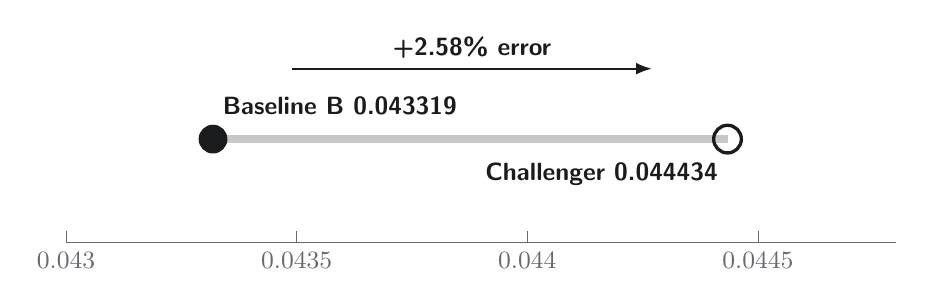
\begin{tikzpicture}
    \begin{axis}[
      width=\textwidth,
      height=45mm,
      xmin=0.0430,
      xmax=0.0448,
      ymin=0.72,
      ymax=1.34,
      axis y line=none,
      axis x line*=bottom,
      ytick=\empty,
      xtick={0.0430,0.0435,0.0440,0.0445},
      scaled x ticks=false,
      x tick label style={font=\small,color=CoverMuted,/pgf/number format/fixed,/pgf/number format/precision=4},
      axis line style={draw=CoverMuted},
      tick style={draw=CoverMuted},
      clip=false
    ]
      \addplot[CoverRule,line width=3pt] coordinates {
        (0.0433186251,1) (0.0444341214,1)
      };
      \addplot[only marks,mark=*,mark size=5pt,CoverInk] coordinates {
        (0.0433186251,1)
      };
      \addplot[only marks,mark=o,mark size=5pt,mark options={line width=1.2pt},CoverInk] coordinates {
        (0.0444341214,1)
      };
      \node[anchor=south west,font=\small\bfseries,text=CoverInk]
        at (axis cs:0.0433186251,1.04) {Baseline B \BaselineBrier};
      \node[anchor=north east,font=\small\bfseries,text=CoverInk]
        at (axis cs:0.0444341214,0.96) {Challenger \ChallengerBrier};
      \draw[-{Latex[length=2mm]},CoverInk,line width=0.7pt]
        (axis cs:0.04349,1.19) -- node[above,font=\small\bfseries,text=CoverInk]
        {+\RelativeWorse\ error} (axis cs:0.04427,1.19);
    \end{axis}
  \end{tikzpicture}\par
  \vspace{-2mm}
  \noindent{\small\color{CoverMuted}
  Bootstrap interval for challenger minus Baseline B:
  [\DeltaLow, \DeltaHigh]. The interval remains entirely above zero.\par}

  \vfill
  \begin{tabularx}{\textwidth}{@{}L{45mm}L{40mm}Y@{}}
    {\scriptsize\bfseries\color{CoverMuted}PREPARED BY} &
    {\scriptsize\bfseries\color{CoverMuted}REPORT DATE} &
    {\scriptsize\bfseries\color{CoverMuted}PROTOCOL}\\
    {\large\bfseries\color{CoverInk}Ashish Pandey} &
    {\large\bfseries\color{CoverInk}June 15, 2026} &
    {\large\bfseries\color{CoverInk}Single locked test pass}\\[4mm]
    \multicolumn{3}{@{}l@{}}{\scriptsize\bfseries\color{CoverMuted}REPRODUCIBLE ARTIFACT}\\[0.5mm]
    \multicolumn{3}{@{}l@{}}{\code{trump-occurrence-sprint-handoff-2026-06-15.zip}}\\
  \end{tabularx}
\end{titlepage}

\pagenumbering{roman}
\setcounter{page}{1}

\section*{Executive Summary}
\addcontentsline{toc}{section}{Executive Summary}

This benchmark evaluates whether transcript-content features improve forecasts of
whether a target word or phrase will appear later in a Rev transcript. The
challenger augments a timing/survival baseline with train-only target-adjacent
content features, a fixed duration-sensitivity term, and validation-fitted
calibration. The evaluation uses chronological transcript-level splits and a single
locked test pass.

\begin{insightbox}{Primary conclusion}
Baseline B generalized better. Its locked-test Brier score was
\metric{\BaselineBrier}, compared with \metric{\ChallengerBrier} for the full
challenger. The challenger therefore increased Brier error by
\metric{\DeltaBrier} (\metric{\RelativeWorse} relative). A 1,000-replicate
bootstrap interval for challenger minus baseline Brier was
\metric{[\DeltaLow, \DeltaHigh]}, entirely above zero.
\end{insightbox}

The negative result is consistent across the primary metric, after-start rows, and
the content ablation. Blanking the prefix produced Brier \BlankedBrier, nearly
identical to the full challenger and still worse than Baseline B. The protocol
therefore returns \textbf{STOP} for this challenger path.

The result is operationally informative rather than merely null. It establishes
that, under this corpus size and temporal shift, local TF--IDF/SVD and adjacency
features do not add reliable out-of-time signal beyond timing and survival. A
future continuation would require a materially different model class or a new
corpus and a newly locked test, rather than tuning against the exposed test set.

\vspace{2mm}
\tableofcontents
\clearpage
\pagenumbering{arabic}
\setcounter{page}{1}

\section{Objective and Task Definition}

\subsection{Forecasting task}
For transcript \(i\), target \(j\), and checkpoint \(t\), the benchmark predicts
the probability that target \(j\) will occur later in the transcript, conditional
on the target not having appeared by checkpoint \(t\):
\[
  p_{ijt} =
  \Pr\!\left(Y_{ijt}=1 \mid \text{target unseen through checkpoint }t\right).
\]
The outcome \(Y_{ijt}\) is one if the target occurs after the checkpoint and zero
otherwise. Checkpoints are replayed over held-out transcripts, yielding multiple
forecast rows per transcript-target pair.

\subsection{Primary decision metric}
The primary metric is mean Brier score:
\[
  \operatorname{Brier}
  = \frac{1}{N}\sum_{n=1}^{N}(p_n-y_n)^2.
\]
Lower values indicate better probabilistic accuracy. Expected calibration error
(ECE), log loss, and AUC are reported as diagnostics. They do not override the
predeclared Brier-based decision rule.

\subsection{Decision rule}
The challenger had to pass validation before the locked test could be opened.
After validation, the test set was evaluated once. Failure to improve on Baseline B
on the full locked-test rows triggers \textbf{STOP}.

\begin{figure}[H]
  \centering
  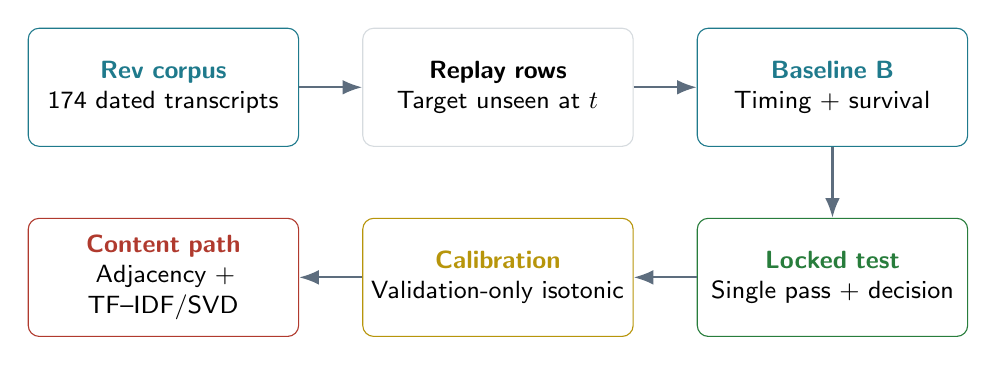
\begin{tikzpicture}[
    node distance=9mm and 8mm,
    box/.style={
      draw=Rule, fill=white, rounded corners=1.4mm,
      minimum height=15mm, text width=32mm, align=center,
      font=\small
    },
    arr/.style={-{Latex[length=2.5mm]}, thick, draw=Muted}
  ]
    \node[box,draw=Teal] (corpus) {\textbf{\color{Teal}Rev corpus}\\174 dated transcripts};
    \node[box,right=of corpus] (replay) {\textbf{Replay rows}\\Target unseen at \(t\)};
    \node[box,right=of replay,draw=Teal] (base) {\textbf{\color{Teal}Baseline B}\\Timing + survival};
    \node[box,below=of corpus,draw=Red] (content) {\textbf{\color{Red}Content path}\\Adjacency + TF--IDF/SVD};
    \node[box,right=of content,draw=Gold] (cal) {\textbf{\color{Gold}Calibration}\\Validation-only isotonic};
    \node[box,right=of cal,draw=Green] (test) {\textbf{\color{Green}Locked test}\\Single pass + decision};

    \draw[arr] (corpus) -- (replay);
    \draw[arr] (replay) -- (base);
    \draw[arr] (base) -- (test);
    \draw[arr] (test) -- (cal);
    \draw[arr] (cal) -- (content);
  \end{tikzpicture}
  \caption{Benchmark execution path and locked-test control.}
\end{figure}

\section{Dataset and Experimental Design}

\subsection{Corpus construction}
The final corpus contains 174 dated Donald Trump transcripts discovered from Rev's
Donald Trump category page and Rev's own sitemap. Raw HTML was saved locally.
Cleaning preferred Donald Trump speaker turns when labeled, otherwise selected a
dominant speaker when reliable, and fell back to all parsed turns when necessary.
Exact normalized text hashes and repeated title/date pairs were deduplicated.

\begin{table}[H]
  \centering
  \caption{Corpus and benchmark scale.}
  \begin{tabularx}{\textwidth}{@{}L{44mm}Y@{}}
    \toprule
    \textbf{Item} & \textbf{Value}\\
    \midrule
    Transcript count & 174 retained transcripts\\
    Corpus date range & July 5, 2019 to June 7, 2026\\
    Transcript length & Median 3,041 words; interquartile range 1,210--6,973\\
    Frozen targets & 180 train-only words or phrases\\
    Target bands & 40 high, 40 mid, 40 rare, 30 cold, 30 phrase\\
    Locked-test rows & 38,790 forecast rows across 26 transcripts\\
    \bottomrule
  \end{tabularx}
\end{table}

\subsection{Chronological split}
The split is chronological and transcript-level: no transcript appears in more
than one split. The validation and test periods are dominated by newer material,
which creates a meaningful temporal generalization test.

\begin{figure}[H]
  \centering
  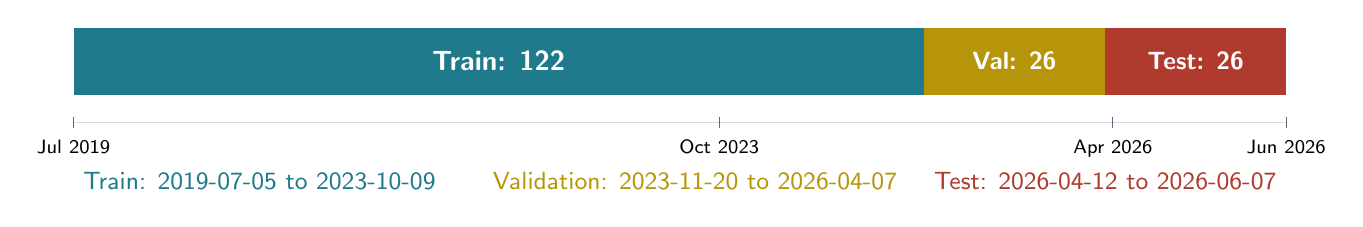
\begin{tikzpicture}
    \def\W{15.4}
    \def\H{0.85}
    \fill[Teal] (0,0) rectangle ({\W*122/174},\H);
    \fill[Gold] ({\W*122/174},0) rectangle ({\W*(122+26)/174},\H);
    \fill[Red] ({\W*(122+26)/174},0) rectangle (\W,\H);
    \node[white,font=\bfseries] at ({\W*61/174},0.425) {Train: 122};
    \node[white,font=\bfseries\small] at ({\W*(122+13)/174},0.425) {Val: 26};
    \node[white,font=\bfseries\small] at ({\W*(148+13)/174},0.425) {Test: 26};

    \draw[Rule] (0,-0.35) -- (\W,-0.35);
    \foreach \x/\lab in {
      0/{Jul 2019},
      8.2/{Oct 2023},
      13.2/{Apr 2026},
      15.4/{Jun 2026}
    }{
      \draw[Muted] (\x,-0.28) -- (\x,-0.43);
      \node[font=\scriptsize,anchor=north] at (\x,-0.45) {\lab};
    }

    \node[anchor=west,font=\small\color{Teal}] at (0,-1.1)
      {Train: 2019-07-05 to 2023-10-09};
    \node[anchor=west,font=\small\color{Gold}] at (5.2,-1.1)
      {Validation: 2023-11-20 to 2026-04-07};
    \node[anchor=east,font=\small\color{Red}] at (\W,-1.1)
      {Test: 2026-04-12 to 2026-06-07};
  \end{tikzpicture}
  \caption{Chronological transcript-level split. Bar width reflects transcript count; dates are annotated below.}
\end{figure}

\begin{table}[H]
  \centering
  \caption{Format distribution by split.}
  \small
  \begin{tabular}{@{}lrrrrrrr@{}}
    \toprule
    \textbf{Split} & \textbf{Interview} & \textbf{Legal} &
    \textbf{Press} & \textbf{Rally} & \textbf{Speech} &
    \textbf{Unknown} & \textbf{Total}\\
    \midrule
    Train & 10 & 4 & 32 & 16 & 23 & 37 & 122\\
    Validation & 0 & 1 & 4 & 4 & 1 & 16 & 26\\
    Locked test & 1 & 0 & 7 & 0 & 1 & 17 & 26\\
    \bottomrule
  \end{tabular}
\end{table}

\subsection{Leakage and freeze controls}
\begin{itemize}
  \item Targets were selected from training data only and frozen before validation and test.
  \item Content features and adjacency statistics were fit using training data only.
  \item Calibration was fit on validation predictions and frozen before the test pass.
  \item Model, corpus, split, target, configuration, and validation artifacts were hashed before test-label use.
  \item The locked test script was run once for the reported decision.
\end{itemize}

\section{Models and Validation Gate}

\begin{table}[H]
  \centering
  \caption{Compared forecasting systems.}
  \begin{tabularx}{\textwidth}{@{}L{38mm}Y@{}}
    \toprule
    \textbf{System} & \textbf{Definition}\\
    \midrule
    Baseline A: constant &
      Forecasts from a fixed occurrence-rate reference.\\
    Baseline B: timing/survival &
      Uses checkpoint timing, exposure, and target survival information without
      transcript-content features.\\
    Challenger full &
      Adds train-only target-adjacent features, trailing and full-prefix TF--IDF/SVD
      representations, and fixed duration sensitivity over Baseline B in logit
      space; calibrated on validation.\\
    Challenger blanked &
      Runs the challenger path with content blanked to estimate whether transcript
      content contributes useful incremental signal.\\
    \bottomrule
  \end{tabularx}
\end{table}

The challenger passed the validation gate: Baseline B validation Brier was
\metric{0.040780}, while challenger Brier was \metric{0.040337}. Duration
sensitivity was directionally valid, with monotonic fraction \metric{0.766} and
mean high-minus-low sensitivity \metric{0.074876}. These checks authorized the
single locked-test pass.

\begin{insightbox}{Why LoRA was not trained}
LoRA was a P1 extension, not the P0 acceptance path. The feature challenger
completed the required validation and locked-test protocol and produced a valid
STOP decision. Training an additional model after opening the locked test would
not change that result and would risk post-test model selection.
\end{insightbox}

\clearpage
\section{Locked-Test Results}

\subsection{Primary metrics}
\begin{table}[H]
  \centering
  \caption{Locked-test performance on 38,790 rows. Lower is better for Brier, ECE, and log loss.}
  \small
  \begin{tabular}{@{}l
    S[table-format=1.6]
    S[table-format=1.6]
    S[table-format=1.6]
    S[table-format=1.6]@{}}
    \toprule
    \textbf{Model} & {\textbf{Brier}} & {\textbf{ECE}} &
    {\textbf{Log loss}} & {\textbf{AUC}}\\
    \midrule
    Constant baseline & 0.048416 & 0.022703 & 0.170778 & 0.923560\\
    \rowcolor{SoftTeal}
    Timing/survival baseline & 0.043319 & 0.018365 & 0.150796 & 0.946593\\
    Challenger full & 0.044434 & 0.018069 & 0.154722 & 0.943082\\
    Challenger blanked & 0.044460 & 0.014503 & 0.155044 & 0.941189\\
    \bottomrule
  \end{tabular}
\end{table}

\begin{figure}[H]
  \centering
  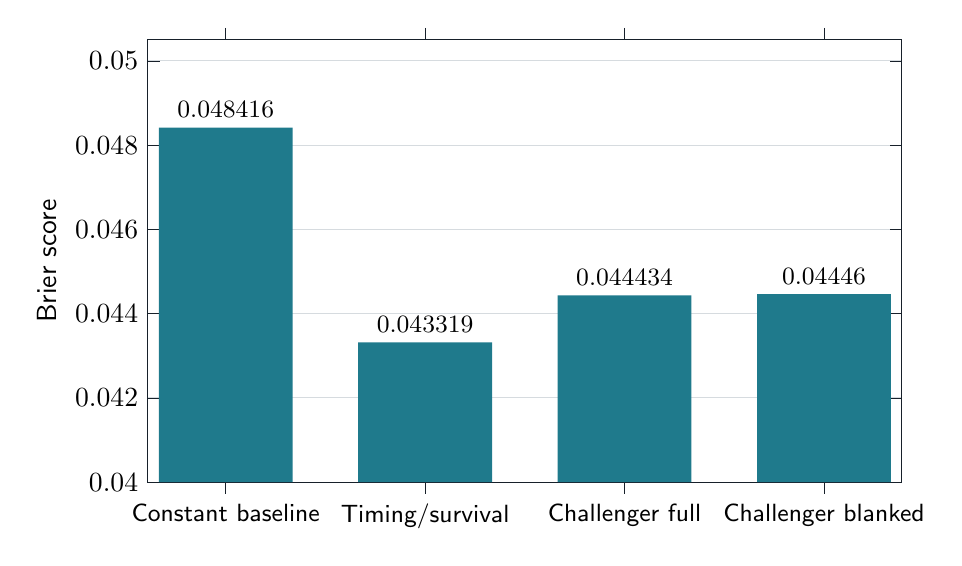
\begin{tikzpicture}
    \begin{axis}[
      width=0.92\textwidth,
      height=72mm,
      ybar,
      bar width=17mm,
      ymin=0.040,
      ymax=0.0505,
      ylabel={Brier score},
      symbolic x coords={Constant,Timing,Full,Blanked},
      xtick=data,
      xticklabels={Constant baseline,Timing/survival,Challenger full,Challenger blanked},
      x tick label style={font=\small,align=center},
      ymajorgrids=true,
      grid style={Rule},
      scaled y ticks=false,
      yticklabel style={/pgf/number format/fixed,/pgf/number format/precision=3},
      axis line style={Ink},
      tick style={Ink},
      nodes near coords,
      nodes near coords style={font=\small\bfseries,anchor=south,/pgf/number format/fixed,/pgf/number format/precision=6},
      enlarge x limits=0.13,
      every axis plot/.append style={draw=none}
    ]
      \addplot[fill=Teal] coordinates {
        (Constant,0.048416)
        (Timing,0.043319)
        (Full,0.044434)
        (Blanked,0.044460)
      };
    \end{axis}
  \end{tikzpicture}
  \caption{Locked-test Brier score. Baseline B is the best-performing system.}
\end{figure}

\subsection{Decision uncertainty}
The observed challenger-minus-baseline Brier delta is
\(\Delta = +\DeltaBrier\). Positive values are unfavorable because they indicate
greater error than Baseline B.

\begin{figure}[H]
  \centering
  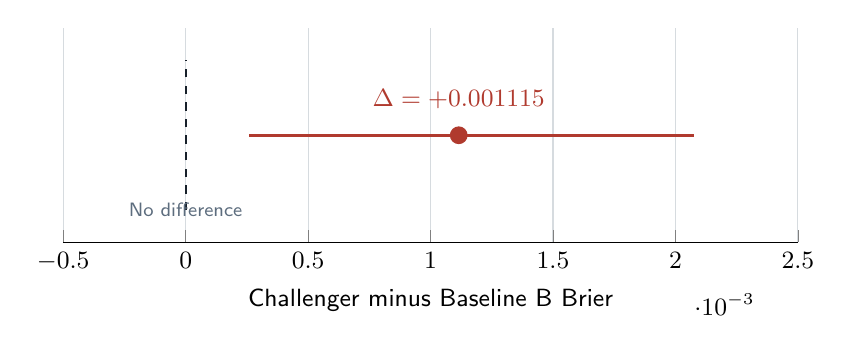
\begin{tikzpicture}
    \begin{axis}[
      width=0.9\textwidth,
      height=43mm,
      xmin=-0.0005,
      xmax=0.0025,
      ymin=0.5,
      ymax=1.5,
      ytick={1},
      yticklabels={Challenger full},
      xlabel={Challenger minus Baseline B Brier},
      xmajorgrids=true,
      grid style={Rule},
      axis y line=none,
      axis x line*=bottom,
      tick label style={font=\small},
      label style={font=\small}
    ]
      \addplot[draw=Red,very thick] coordinates {(\DeltaLow,1) (\DeltaHigh,1)};
      \addplot[Red,only marks,mark=*,mark size=3pt] coordinates {(\DeltaBrier,1)};
      \draw[Ink,dashed,thick] (axis cs:0,0.65) -- (axis cs:0,1.35);
      \node[anchor=south,font=\small\bfseries\color{Red}] at (axis cs:\DeltaBrier,1.08)
        {\(\Delta=+\DeltaBrier\)};
      \node[anchor=north,font=\scriptsize\color{Muted}] at (axis cs:0,0.73)
        {No difference};
    \end{axis}
  \end{tikzpicture}
  \caption{Bootstrap 95\% interval from 1,000 transcript-level replicates. The entire interval is above zero.}
\end{figure}

\begin{decisionbox}
  \textbf{Decision interpretation.}
  Baseline B outperformed the challenger on the primary metric. The bootstrap
  interval does not include zero, and the direction is unfavorable throughout.
  The first STOP condition is therefore met.
\end{decisionbox}

\clearpage
\section{Calibration and Ablation Diagnostics}

\subsection{Calibration and loss profile}
\begin{figure}[H]
  \centering
  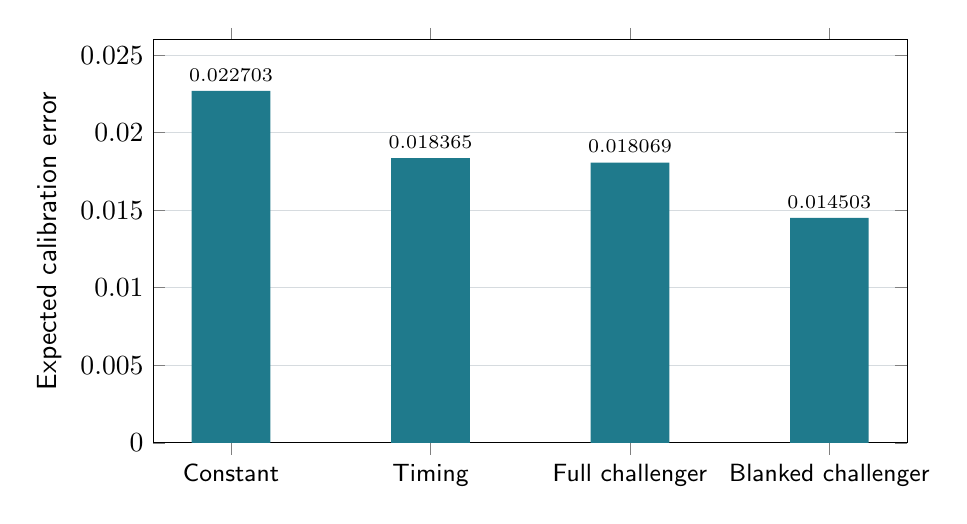
\begin{tikzpicture}
    \begin{axis}[
      width=0.92\textwidth,
      height=67mm,
      ybar,
      bar width=10mm,
      ymin=0,
      ymax=0.026,
      ylabel={Expected calibration error},
      symbolic x coords={Constant,Timing,Full,Blanked},
      xtick=data,
      xticklabels={Constant,Timing,Full challenger,Blanked challenger},
      x tick label style={font=\small,align=center},
      ymajorgrids=true,
      grid style={Rule},
      scaled y ticks=false,
      yticklabel style={/pgf/number format/fixed,/pgf/number format/precision=3},
      nodes near coords,
      nodes near coords style={font=\scriptsize\bfseries,anchor=south,/pgf/number format/fixed,/pgf/number format/precision=6},
      enlarge x limits=0.13,
      every axis plot/.append style={draw=none}
    ]
      \addplot[fill=Teal] coordinates {
        (Constant,0.022703)
        (Timing,0.018365)
        (Full,0.018069)
        (Blanked,0.014503)
      };
    \end{axis}
  \end{tikzpicture}
  \caption{Expected calibration error. Calibration is acceptable but does not offset worse Brier performance.}
\end{figure}

\subsection{Reliability curves}
\begin{figure}[H]
  \centering
  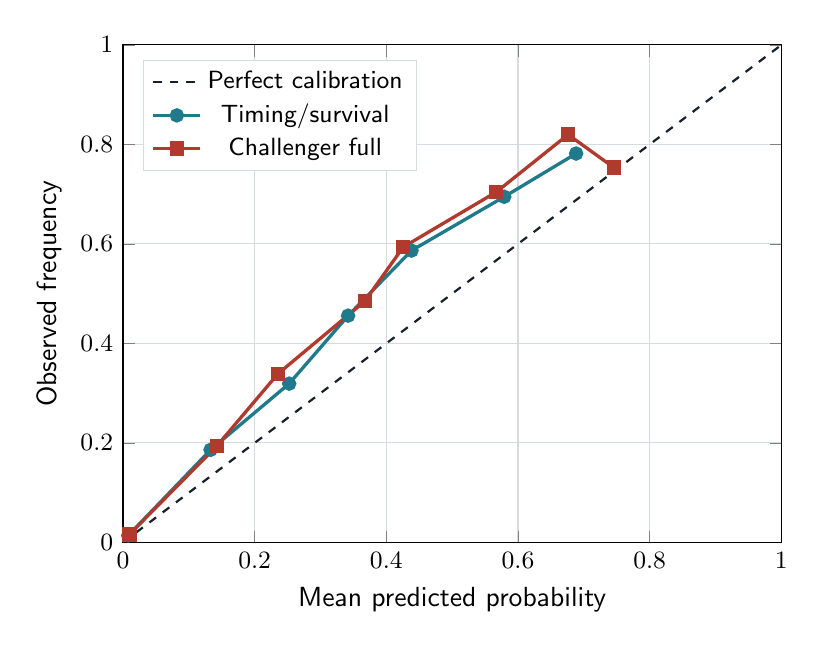
\begin{tikzpicture}
    \begin{axis}[
      width=0.82\textwidth,
      height=79mm,
      xmin=0,xmax=1,
      ymin=0,ymax=1,
      xlabel={Mean predicted probability},
      ylabel={Observed frequency},
      grid=both,
      grid style={Rule},
      legend style={at={(0.03,0.97)},anchor=north west,draw=Rule,fill=white,font=\small},
      tick label style={font=\small}
    ]
      \addplot[Ink,dashed,thick,domain=0:1] {x};
      \addlegendentry{Perfect calibration}
      \addplot[Teal,very thick,mark=*,mark size=2pt]
        coordinates {
          (0.008097,0.014058)
          (0.133023,0.186117)
          (0.252442,0.319196)
          (0.341973,0.455801)
          (0.438227,0.586667)
          (0.579044,0.694737)
          (0.688270,0.781687)
        };
      \addlegendentry{Timing/survival}
      \addplot[Red,very thick,mark=square*,mark size=2pt]
        coordinates {
          (0.009676,0.015994)
          (0.142571,0.193914)
          (0.235319,0.338912)
          (0.367331,0.484772)
          (0.425642,0.593674)
          (0.566885,0.704225)
          (0.676056,0.819788)
          (0.745448,0.753597)
        };
      \addlegendentry{Challenger full}
    \end{axis}
  \end{tikzpicture}
  \caption{Reliability curves using populated probability bins. The extreme challenger bin with seven observations is omitted from the plot but retained in the metric calculation.}
\end{figure}

\subsection{Content ablation}
\begin{figure}[H]
  \centering
  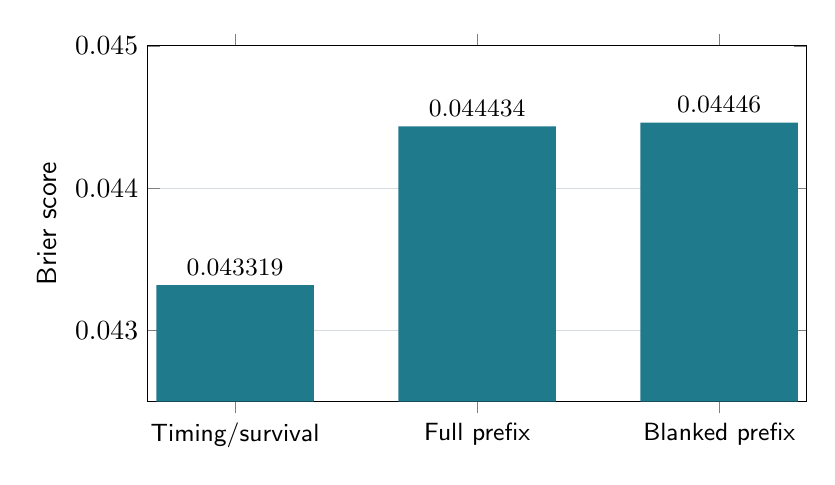
\begin{tikzpicture}
    \begin{axis}[
      width=0.82\textwidth,
      height=61mm,
      ybar,
      bar width=20mm,
      ymin=0.0425,
      ymax=0.0450,
      ylabel={Brier score},
      symbolic x coords={Timing,Full,Blanked},
      xtick=data,
      xticklabels={Timing/survival,Full prefix,Blanked prefix},
      x tick label style={font=\small,align=center},
      ymajorgrids=true,
      grid style={Rule},
      scaled y ticks=false,
      yticklabel style={/pgf/number format/fixed,/pgf/number format/precision=3},
      nodes near coords,
      nodes near coords style={font=\small\bfseries,anchor=south,/pgf/number format/fixed,/pgf/number format/precision=6},
      enlarge x limits=0.18,
      every axis plot/.append style={draw=none}
    ]
      \addplot[fill=Teal] coordinates {
        (Timing,0.043319)
        (Full,0.044434)
        (Blanked,0.044460)
      };
    \end{axis}
  \end{tikzpicture}
  \caption{Content ablation. Full-prefix and blanked-prefix variants are nearly identical and both trail Baseline B.}
\end{figure}

The ablation does not support a useful test-time content contribution. On rows with
\(t>0\), Baseline B achieved Brier \metric{0.039284}, while the full challenger
achieved \metric{0.040592}. Thus, the challenger remains worse after the transcript
has begun, not only at the initial checkpoint.

\section{Decision, Limitations, and Next-Step Boundary}

\subsection{Evidence-to-decision matrix}
\begin{table}[H]
  \centering
  \caption{Predeclared decision evidence.}
  \small
  \begin{tabularx}{\textwidth}{@{}L{34mm}Y L{34mm}@{}}
    \toprule
    \textbf{Check} & \textbf{Evidence} & \textbf{Interpretation}\\
    \midrule
    Primary Brier &
      Challenger \ChallengerBrier\ vs Baseline B \BaselineBrier &
      Fails continuation bar\\
    Bootstrap interval &
      Challenger-minus-baseline CI [\DeltaLow, \DeltaHigh] &
      Entirely unfavorable\\
    Content ablation &
      Full \ChallengerBrier; blanked \BlankedBrier &
      No useful content lift\\
    After-start rows &
      Baseline 0.039284; challenger 0.040592 &
      Supports STOP\\
    Calibration &
      Challenger ECE 0.018069 vs baseline 0.018365 &
      Similar; cannot override Brier\\
    Cost and latency &
      \$0 API cost; 0.000890 s per validation prediction after feature construction &
      Operationally feasible\\
    \bottomrule
  \end{tabularx}
\end{table}

\subsection{Limitations}
\begin{itemize}
  \item \textbf{Temporal shift.} The locked test is concentrated in newer, shorter
    2026 press/event transcripts. This is the intended out-of-time challenge but
    may penalize train-only lexical features.
  \item \textbf{Speaker extraction.} Primary-speaker extraction is heuristic when
    Rev labels are missing or ambiguous.
  \item \textbf{Content model class.} The tested challenger is TF--IDF/SVD plus
    target-adjacent statistics, not a fine-tuned language model.
  \item \textbf{Contamination probe.} A deterministic local \code{distilgpt2}
    screen flagged zero test transcripts. This is not proof that no public
    transcript occurs in a larger model's pretraining data.
  \item \textbf{Single test pass.} The test set is now exposed and cannot be used
    for further model selection without invalidating the original protocol.
\end{itemize}

\subsection{Bounded next step}
The appropriate conclusion is to stop this specific challenger path. A new attempt
would require one of the following before any new locked evaluation:
\begin{enumerate}
  \item a materially larger or more diverse transcript corpus;
  \item a different representation or model class with stronger temporal transfer;
  \item a new target construction strategy; and
  \item a newly reserved chronological test period.
\end{enumerate}
Tuning against the current test outcomes is not a valid continuation.

\section{Reproducibility Record}

\begin{table}[H]
  \centering
  \caption{Primary package records.}
  \begin{tabularx}{\textwidth}{@{}L{43mm}Y@{}}
    \toprule
    \textbf{Artifact} & \textbf{Record}\\
    \midrule
    Handoff package &
      \code{trump-occurrence-sprint-handoff-2026-06-15.zip}\\
    Package SHA256 &
      \begingroup\ttfamily\footnotesize\PackageHash\endgroup\\
    Final decision &
      \code{DECISION.md}\\
    Primary test metrics &
      \code{metrics/test\_metrics.json}\\
    Bootstrap results &
      \code{metrics/bootstrap\_deltas.json}\\
    Freeze manifest &
      \code{metrics/freeze\_manifest.json}\\
    Data card &
      \code{data/data\_card.md}\\
    Model artifacts &
      \code{models/baselines.pkl}, \code{models/challenger.pkl}\\
    \bottomrule
  \end{tabularx}
\end{table}

\subsection{Reproduction sequence}
\begin{tcblisting}{
  listing only,
  colback=SoftGray,
  colframe=Rule,
  boxrule=0.5pt,
  arc=1mm,
  left=3mm,right=3mm,top=2mm,bottom=2mm,
  listing options={
    basicstyle=\ttfamily\small,
    columns=fullflexible,
    breaklines=true,
    showstringspaces=false
  }
}
py -3 -m pip install -r requirements.txt
py -3 -m pytest tests
py -3 -m src.run_phase0
py -3 -m src.run_phase1
py -3 -m src.run_phase2
py -3 -m src.run_phase3
py -3 -m src.run_phase4_locked_test
\end{tcblisting}

\textbf{Protocol warning.} The final command is the single locked-test pass. It
should not be rerun for model selection after inspecting the reported test metrics.

\subsection{Integrity statement}
The handoff archive contains 245 entries, including 180 saved raw HTML artifacts.
The archive checksum matches its sidecar file. Frozen model, configuration, corpus,
split, target, and validation artifacts match the hashes recorded in the freeze
manifest. The sprint test suite passes 11 tests.

\vfill
\begin{center}
  \color{Muted}\small
  End of technical report
\end{center}

\end{document}
